% answers.tex —— 1995 年·上海卷·文史类 · 参考答案与详细解析片段
% 由 tools/generate_projects.py 依来源总账自 1995/1995_数学真题_上海文_试题.md + 1995/1995_数学真题_上海文_解析正文.md + 1995/1995_数学真题_上海文_答案要点.md 生成，勿手改（改源 MD 后重跑）


\begin{gktip}
卷内答案和步骤来自同一固定扫描件，出版者/版次及其官方身份未核。以下按题面重新核算；不把转录的卷内答案当作数学正确性的唯一依据。$A_1/B_1$、$A_2/B_2$ 是原卷选做轨道。
\end{gktip}

\gkpart{选择题}

\begin{answer}
\gksolhead{1}{答案 C}

\textbf{题目}：

$y=\sin^2x$ 是\mbox{（　　）}

（A）最小正周期为 $2\pi$ 的偶函数　（B）最小正周期为 $2\pi$ 的奇函数

（C）最小正周期为 $\pi$ 的偶函数　（D）最小正周期为 $\pi$ 的奇函数

\Needspace{4\baselineskip}
\textbf{解析}

$\sin^2x=\dfrac{1-\cos2x}{2}$，是偶函数，最小正周期为 $\pi$。

\gkanswer{答案：C。}

\end{answer}
\begin{answer}
\gksolhead{2}{答案 B}

\textbf{题目}：

如果 $P=\{x\mid(x-1)(2x-5)<0\}$，$Q=\{x\mid0<x<10\}$，那么\mbox{（　　）}

（A）$P\cap Q=\varnothing$　　（B）$P\subset Q$　　（C）$P\supset Q$　　（D）$P\cup Q=\mathbb R$

\Needspace{4\baselineskip}
\textbf{解析}

$(x-1)(2x-5)<0$ 的解集是 $P=(1,\frac52)$。又 $Q=(0,10)$，所以 $P\subset Q$。

\gkanswer{答案：B。}

\end{answer}
\begin{answer}
\gksolhead{3}{答案 B}

\textbf{题目}：

方程 $\tan\left(2x+\dfrac\pi3\right)=\dfrac{\sqrt3}{3}$ 在区间 $[0,2\pi)$ 上解的个数是\mbox{（　　）}

\begin{gkopts}(4)
\task （A）5
\task （B）4
\task （C）3
\task （D）2
\end{gkopts}

\Needspace{4\baselineskip}
\textbf{解析}

$\tan u=\dfrac{\sqrt3}{3}$ 当且仅当 $u=\dfrac\pi6+k\pi$。令 $u=2x+\dfrac\pi3$，得 $x=-\dfrac\pi{12}+k\dfrac\pi2$。在 $[0,2\pi)$ 内对应 $k=1,2,3,4$，共有 4 个解。

\gkanswer{答案：B。}

\end{answer}
\begin{answer}
\gksolhead{4}{答案 C}

\textbf{题目}：

设棱锥的底面面积是 $8\,\mathrm{cm}^2$，那么这个棱锥的中截面（过棱锥高的中点\allowbreak 且平行于底面的截面）的面积是\allowbreak\mbox{（　　）}

（A）$4\,\mathrm{cm}^2$　　（B）$2\sqrt2\,\mathrm{cm}^2$　　（C）$2\,\mathrm{cm}^2$　　（D）$\sqrt2\,\mathrm{cm}^2$

\Needspace{4\baselineskip}
\textbf{解析}

过棱锥高的中点且平行底面的截面与底面相似，线性比为 $1:2$，面积比为 $1:4$。截面面积为 $8/4=2\,\mathrm{cm}^2$。

\gkanswer{答案：C。}

\end{answer}
\begin{answer}
\gksolhead{5}{答案 A}

\textbf{题目}：

“$ab<0$”是“方程 $ax^2+by^2=c$ 表示双曲线”的\mbox{（　　）}

（A）必要条件但不是充分条件　（B）充分条件但不是必要条件

（C）充分必要条件　（D）既不是充分条件又不是必要条件

\Needspace{4\baselineskip}
\textbf{解析}

若 $ax^2+by^2=c$ 表示双曲线，二次项系数必须异号，故 $ab<0$ 是必要条件。它不是充分条件：例如 $c=0$ 时曲线退化为两条相交直线，不是非退化双曲线。

\gkanswer{答案：A。}

\end{answer}
\begin{answer}
\gksolhead{6}{答案 A}

\textbf{题目}：

当 $a\ne0$ 时，函数 $y=ax+b$ 和 $y=b^{ax}$ 的图象只可能是\mbox{（　　）}
\nopagebreak[4]
\begin{center}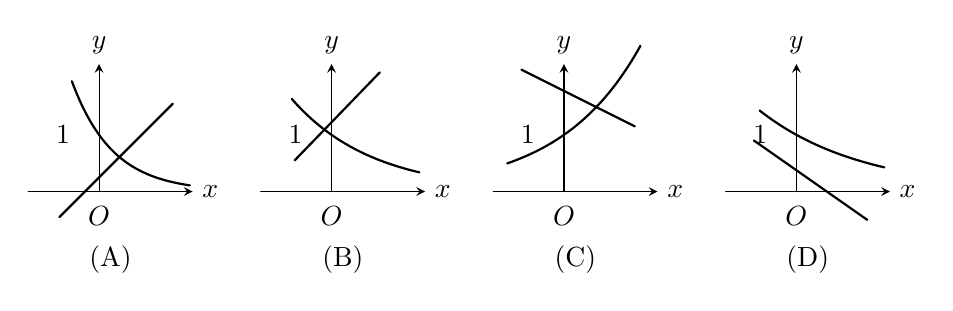
\begin{tikzpicture}[>=stealth,scale=0.72,line cap=round,line join=round]
\foreach \x/\name in {0/A,4.1/B,8.2/C,12.3/D}{
  \begin{scope}[shift={(\x,0)}]
    \draw[->] (-1.25,0)--(1.65,0) node[right] {$x$};
    \draw[->] (0,0)--(0,2.25) node[above] {$y$};
    \node[left=7pt] at (0,1) {$1$};
    \node[below=2pt] at (0,0) {$O$};
    \node at (0.2,-1.2) {(\name)};
  \end{scope}
}
% A: a>0 and 0<b<1; both curves use the same a,b.
\begin{scope}[shift={(0,0)}]
  \draw[thick,domain=-0.48:1.6,samples=80] plot (\x,{0.25^\x});
  \draw[thick] (-0.7,-0.45)--(1.3,1.55);
\end{scope}
% Distractor sketches retain the qualitative alternatives printed in the source.
\begin{scope}[shift={(4.1,0)}]
  \draw[thick,domain=-0.7:1.55,samples=80] plot (\x,{exp(-0.7*\x)});
  \draw[thick] (-0.65,0.55)--(0.85,2.10);
\end{scope}
\begin{scope}[shift={(8.2,0)}]
  \draw[thick,domain=-1.0:1.35,samples=80] plot (\x,{exp(0.7*\x)});
  \draw[thick] (-0.75,2.15)--(1.25,1.15);
\end{scope}
\begin{scope}[shift={(12.3,0)}]
  \draw[thick,domain=-0.65:1.55,samples=80] plot (\x,{exp(-0.55*\x)});
  \draw[thick] (-0.75,0.90)--(1.25,-0.50);
\end{scope}
\end{tikzpicture}
\end{center}
\nopagebreak[4]
\Needspace{4\baselineskip}
\textbf{解析}

指数曲线 $y=b^{ax}$ 恒正且过 $(0,1)$。A 图中的直线斜率为正、截距在 $0$ 与 $1$ 之间，对应 $a>0,0<b<1$，此时 $b^{ax}$ 随 $x$ 递减，符合图示。其他图的直线斜率、截距与指数曲线增减方向不相容。

\gkanswer{答案：A。}

\end{answer}
\begin{answer}
\gksolhead{7}{答案 D}

\textbf{题目}：

当 $0<a<b<1$ 时，下列不等式中正确的是\mbox{（　　）}

（A）$(1-a)^{1/b}>(1-a)^b$

（B）$(1+a)^a>(1+b)^b$

（C）$(1-a)^b>(1-a)^{b/2}$

（D）$(1-a)^a>(1-b)^b$

\Needspace{4\baselineskip}
\textbf{解析}

$0<a<b<1$ 时，$1-a>1-b>0$。并且 $0<1-b<1$，有 $(1-b)^b<(1-b)^a$；另一方面 $1-a>1-b$，所以 $(1-a)^a>(1-b)^a>(1-b)^b$，D 正确。A、C 的底数小于 1，指数大小关系方向与所列不等式相反；B 也不成立。

\gkanswer{答案：D。}

\end{answer}
\begin{answer}
\gksolhead{8}{答案 B}

\textbf{题目}：

下列四个命题中的真命题是\mbox{（　　）}

（A）经过定点 $P_0(x_0,y_0)$ 的直线都可以用方程 $y-y_0=k(x-x_0)$ 表示。

（B）经过任意两个不同的点 $P_1(x_1,y_1)$、$P_2(x_2,y_2)$ 的直线都可以用方程 $(y-y_1)(x_2-x_1)=(x-x_1)(y_2-y_1)$ 表示。

（C）不经过原点的直线都可以用方程 $\dfrac xa+\dfrac yb=1$ 表示。

（D）经过定点 $A(0,b)$ 的直线都可以用方程 $y=kx+b$ 表示。

\Needspace{4\baselineskip}
\textbf{解析}

A 漏掉竖直直线；C 漏掉平行于坐标轴且不经过原点的直线；D 漏掉过 $A(0,b)$ 的竖直直线。B 的等式对任意两点的横、纵坐标差都成立，并能表示竖直情形，故 B 正确。

\gkanswer{答案：B。}

\end{answer}
\gkpart{填空题}

\begin{answer}
\gksolhead{9}{答案 $x<-3$ 或 $x>4$}

\textbf{题目}：

不等式 $\dfrac{2x-1}{x+3}>1$ 的解是 \gkblank{}。

\Needspace{4\baselineskip}
\textbf{解析}

移项得 $\dfrac{x-4}{x+3}>0$，临界点为 $-3,4$，作符号分析并排除 $x=-3$，得到 $(-\infty,-3)\cup(4,+\infty)$。

\gkanswer{答案：$x<-3$ 或 $x>4$。}

\end{answer}
\begin{answer}
\gksolhead{10}{答案 $3x+4y=0$、$3x-4y=0$}

\textbf{题目}：

双曲线 $\dfrac{x^2}{2}-\dfrac{8y^2}{9}=8$ 的渐近线方程是 \gkblank{}。

\Needspace{4\baselineskip}
\textbf{解析}

原方程化为 $\dfrac{x^2}{16}-\dfrac{y^2}{9}=1$，故渐近线为 $y=\pm\dfrac34x$。

\gkanswer{答案：$3x+4y=0$ 和 $3x-4y=0$。}

\end{answer}
\begin{answer}
\gksolhead{11}{答案 $y=54.8(1+x/100)^8$}

\textbf{题目}：

1992 年底世界人口达到 54.8 亿，若人口的年平均增长率为 $x\%$，2000 年底世界人口数为 $y$（亿），那么 $y$ 与 $x$ 的函数关系式是 \gkblank{}。

\Needspace{4\baselineskip}
\textbf{解析}

从 1992 年底到 2000 年底共 8 年，每年增长因子为 $1+x/100$，故 $y=54.8(1+x/100)^8$。

\gkanswer{答案：$y=54.8\left(1+\dfrac{x}{100}\right)^8$。}

\end{answer}
\begin{answer}
\gksolhead{12}{答案 $1$}

\textbf{题目}：

已知 $\log_3x=-\dfrac1{\log_2 3}$，那么 $x+x^2+x^3+\cdots+x^n+\cdots=$ \gkblank{}。

\Needspace{4\baselineskip}
\textbf{解析}

由换底公式，$\log_3x=-\log_3 2$，所以 $x=1/2$。所求无穷等比级数和为 $\dfrac{x}{1-x}=1$。

\gkanswer{答案：$1$。}

\end{answer}
\begin{answer}
\gksolhead{13}{答案 $11$}

\textbf{题目}：

若 $(x+1)^n=x^n+\cdots+ax^3+bx^2+\cdots+1$（$n\in\mathbb N$），且 $a:b=3:1$，那么 $n=$ \gkblank{}。

\Needspace{4\baselineskip}
\textbf{解析}

二项式展开中 $a=\binom n3$、$b=\binom n2$。于是 $a:b=(n-2):3=3:1$，得 $n=11$。

\gkanswer{答案：$11$。}

\end{answer}
\begin{answer}
\gksolhead{14}{答案 $y^2=-8x+8$}

\textbf{题目}：

到点 $A(-1,0)$ 和直线 $x=3$ 距离相等的点的轨迹方程是 \gkblank{}。

\Needspace{4\baselineskip}
\textbf{解析}

设动点为 $(x,y)$。它到焦点 $(-1,0)$ 与准线 $x=3$ 距离相等，即 $\sqrt{(x+1)^2+y^2}=|x-3|$。平方整理得 $y^2=-8x+8$。

\gkanswer{答案：$y^2=-8x+8$。}

\end{answer}
\begin{answer}
\gksolhead{15}{答案 $y=-\sqrt{(x-1)/3}$，$x\ge1$}

\textbf{题目}：

函数 $y=3x^2+1\;(x\le0)$ 的反函数是 $y=$ \gkblank{}。

\Needspace{4\baselineskip}
\textbf{解析}

原函数定义域为 $x\le0$，值域为 $y\ge1$。由 $x=3y^2+1$ 且反函数值域要求 $y\le0$，得 $y=-\sqrt{(x-1)/3}$，定义域 $x\ge1$。

\gkanswer{答案：$y=-\sqrt{\dfrac{x-1}{3}}$，$x\ge1$。}

\end{answer}
\begin{answer}
\gksolhead{16}{答案 $(\lg2,+\infty)$}

\textbf{题目}：

函数 $y=\lg\sqrt{10^x-2}$ 的定义域是 \gkblank{}。

\Needspace{4\baselineskip}
\textbf{解析}

对数真数要求 $\sqrt{10^x-2}>0$，即 $10^x-2>0$，等价于 $x>\lg2$。

\gkanswer{答案：$(\lg2,+\infty)$。}

\end{answer}
\begin{answer}
\gksolhead{17}{答案 $[-3\pi/2,\pi/2]$}

\textbf{题目}：

函数 $y=\sin\dfrac x2+\cos\dfrac x2$ 在 $(-2\pi,2\pi)$ 内的递增区间是 \gkblank{}。

\Needspace{4\baselineskip}
\textbf{解析}

$y=\sqrt2\sin(x/2+\pi/4)$，且 $y'=\dfrac12(\cos(x/2)-\sin(x/2))$。在原定义域 $(-2\pi,2\pi)$ 内，导数非负的最大连续区间为 $[-3\pi/2,\pi/2]$。端点包含在原定义域内，端点导数为零，函数在该闭区间仍严格递增。

\gkanswer{答案：$\left[-\dfrac{3\pi}{2},\dfrac\pi2\right]$。}

\end{answer}
\begin{answer}
\gksolhead{18}{$A_1$组答案 $-2<r<0$；$B_1$组答案 $e$}

\textbf{题目}：

$A_1$组：若 $\displaystyle\lim_{n\to\infty}\left[1+(r+1)^n\right]=1$，则 $r$ 的取值范围是 \gkblank{}。

$B_1$组：$\displaystyle\lim_{n\to\infty}\left(1+\dfrac1n\right)^{n-2}=$ \gkblank{}。

\Needspace{4\baselineskip}
\textbf{解析}

$A_1$组：要求 $(r+1)^n\to0$，当且仅当 $|r+1|<1$，故 $-2<r<0$。

$B_1$组：$\left(1+\dfrac1n\right)^{n-2}=\left(1+\dfrac1n\right)^n\left(1+\dfrac1n\right)^{-2}\to e$。

\gkanswer{答案：$A_1$组$-2<r<0$。$B_1$组答案：$e$。}

\end{answer}
\begin{answer}
\gksolhead{19}{$A_1$组答案 $350$；$B_1$组答案 $25/33$}

\textbf{题目}：

$A_1$组：从 6 台原装计算机和 5 台组装计算机中任意选取 5 台，其中至少有原装与组装计算机各 2 台，则不同的选取法有 \gkblank{} 种。（结果用数值表示）

$B_1$组：从 6 台原装计算机和 5 台组装计算机中任意选取 5 台，其中至少有原装与组装计算机各 2 台的概率是 \gkblank{}。

\Needspace{4\baselineskip}
\textbf{解析}

合格选法按原装机数量分两类：$\binom62\binom53+\binom63\binom52=150+200=350$。所有选法有 $\binom{11}5=462$ 种，故概率为 $350/462=25/33$。

\gkanswer{答案：$A_1$组$350$ 种。$B_1$组答案：$\dfrac{25}{33}$（或 $0.76$）。}

\end{answer}
\begin{answer}
\gksolhead{20}{$A_1$组答案约 $37.70\,\mathrm{dm}^3$；$B_1$组答案 14 天}

\textbf{题目}：

$A_1$组：把圆心角为 $216^\circ$、半径为 5 分米的扇形铁皮焊成一个圆锥形容器（不计焊缝），那么容器的容积是 \gkblank{} 立方分米。（结果保留两位小数）

$B_1$组：某工程由下列工序组成：工序 $a$ 无紧前工序；$b,c$ 的紧前工序均为 $a$；$d$ 的紧前工序为 $b$；$e$ 的紧前工序为 $c,d$。工时数（天）分别为 $a:2,b:3,c:5,d:6,e:3$。那么工程总时数是 \gkblank{} 天。

\Needspace{4\baselineskip}
\textbf{解析}

$A_1$组：扇形弧长为 $5\cdot216^\circ\cdot\pi/180^\circ=6\pi$ 分米，焊成圆锥后底面半径为 3 分米，母线为 5 分米，高为 4 分米。因此体积 $V=\dfrac13\pi\cdot3^2\cdot4=12\pi\approx37.70\,\mathrm{dm}^3$。原评分标准接受 37.68 或 37.69。

$B_1$组：关键路径为 $a\to b\to d\to e$，时长 $2+3+6+3=14$ 天；另一支 $a\to c\to e$ 为 $2+5+3=10$ 天，故总工时为 14 天。

\gkanswer{答案：$A_1$组$37.70\,\mathrm{dm}^3$；原评分标准接受 $37.68$ 或 $37.69$。$B_1$组答案：$14$ 天。}

\end{answer}
\gkpart{解答题}

\begin{answer}
\gksolhead{21}{$A_2$组答案 $-4/5$；$B_2$组答案见下}

\textbf{题目}：

$A_2$组（本题满分 12 分）：已知 $\tan\left(\dfrac\pi4+\theta\right)=3$，求 $\sin2\theta-2\cos^2\theta$ 的值。

$B_2$组（本题满分 12 分，共 2 小题，第 1 小题满分 4 分，第 2 小题满分 8 分）：如图，在空间直角坐标系中，$BC=2$，原点 $O$ 是 $BC$ 的中点，点 $A$ 的坐标是 $\left(\dfrac{\sqrt3}{2},\dfrac12,0\right)$，点 $D$ 在平面 $yoz$ 上，且 $\angle BDC=90^\circ$，$\angle DCB=30^\circ$。
\nopagebreak[4]
\begin{center}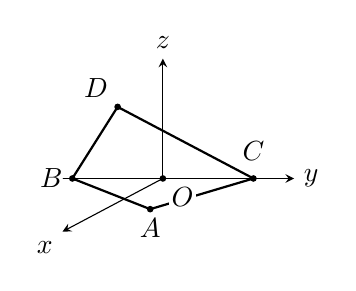
\begin{tikzpicture}[
  x={(-0.85cm,-0.45cm)}, y={(1.15cm,0cm)}, z={(0cm,1.05cm)},
  >=stealth,scale=1.0,line cap=round,line join=round]
  \coordinate (O) at (0,0,0);
  \coordinate (B) at (0,-1,0);
  \coordinate (C) at (0,1,0);
  \coordinate (A) at ({sqrt(3)/2},0.5,0);
  \coordinate (D) at (0,-0.5,{sqrt(3)/2});
  \draw[->] (O)--(1.5,0,0) node[below left] {$x$};
  \draw[->] (0,-1.1,0)--(0,1.45,0) node[right] {$y$};
  \draw[->] (O)--(0,0,1.45) node[above] {$z$};
  \draw[thick] (B)--(D)--(C)--(A)--cycle;
  \fill (O) circle (1.2pt) node[fill=white,inner sep=1pt,below right=2pt] {$O$};
  \fill (A) circle (1.2pt) node[below] {$A$};
  \fill (B) circle (1.2pt) node[left] {$B$};
  \fill (C) circle (1.2pt) node[above=3pt] {$C$};
  \fill (D) circle (1.2pt) node[above left] {$D$};
\end{tikzpicture}
\end{center}
\nopagebreak[4]
（1）求向量 $\overrightarrow{OD}$ 的坐标；（2）设向量 $\overrightarrow{AD}$ 和 $\overrightarrow{BC}$ 的夹角为 $\theta$，求 $\cos\theta$ 的值。

\Needspace{4\baselineskip}
\textbf{解析}

\Needspace{5\baselineskip}
$A_2$组：由正切和角公式，$\tan\theta=\dfrac{3-1}{1+3}=\dfrac12$。因此
\nopagebreak[4]
\[
\sin2\theta-2\cos^2\theta=\frac{2\tan\theta-2}{1+\tan^2\theta}=-\frac45.
\]

$B_2$组：取 $B=(0,-1,0)$、$C=(0,1,0)$。在直角三角形 $BDC$ 中 $BC=2$ 为斜边，且 $\angle DCB=30^\circ$，故 $DC=\sqrt3$、$DB=1$。结合 $D\in yoz$ 平面及原图位置，$D=(0,-1/2,\sqrt3/2)$，所以 $\overrightarrow{OD}=(0,-1/2,\sqrt3/2)$。

\Needspace{5\baselineskip}
$\overrightarrow{AD}=(-\sqrt3/2,-1,\sqrt3/2)$，$\overrightarrow{BC}=(0,2,0)$。于是 $\overrightarrow{AD}\cdot\overrightarrow{BC}=-2$，$|AD|=\sqrt{5/2}$，$|BC|=2$，从而
\nopagebreak[4]
\[
\cos\theta=\frac{-2}{2\sqrt{5/2}}=-\frac{\sqrt{10}}5.
\]

\gkanswer{答案：$A_2$组$-\dfrac45$。$B_2$组答案：（1）$\overrightarrow{OD}=\left(0,-\dfrac12,\dfrac{\sqrt3}{2}\right)$；（2）$\cos\theta=-\dfrac{\sqrt{10}}5$。}

\end{answer}
\begin{answer}
\gksolhead{22}{$A_2$组答案见下；$B_2$组答案 $f(x)=(x+1)^2$、面积 $1/3$}

\textbf{题目}：

$A_2$组（本题满分 14 分）：已知复数 $z_1,z_2$ 满足 $|z_1|=|z_2|=1$，且 $z_1+z_2=i$，求 $z_1,z_2$ 的值。

$B_2$组（本题满分 14 分，共 2 小题，第 1 小题满分 7 分，第 2 小题满分 7 分）：设 $y=f(x)$ 是二次函数，方程 $f(x)=0$ 有两个相等的实根，且 $f'(x)=2x+2$。（1）求 $y=f(x)$ 的表达式；（2）求 $y=f(x)$ 的图象与两坐标轴所围成图形的面积。

\Needspace{4\baselineskip}
\textbf{解析}

$A_2$组：令 $z_1=a+bi$、$z_2=-a+(1-b)i$。由 $|z_1|=|z_2|=1$ 得 $a^2+b^2=a^2+(1-b)^2=1$，故 $b=1/2$、$a=\pm\sqrt3/2$。因此两数为 $\sqrt3/2+i/2$ 与 $-\sqrt3/2+i/2$，次序可互换。

\Needspace{5\baselineskip}
$B_2$组：设 $f(x)=ax^2+bx+c$。由 $f'(x)=2x+2$ 得 $a=1,b=2$。判别式为零，$b^2-4ac=0$，故 $c=1$，即 $f(x)=(x+1)^2$。图象与两坐标轴围成的面积是
\nopagebreak[4]
\[
\int_{-1}^{0}(x+1)^2\,dx=\frac13.
\]

\gkanswer{答案：$A_2$组$(z_1,z_2)=\left(\dfrac{\sqrt3}{2}+\dfrac12i,-\dfrac{\sqrt3}{2}+\dfrac12i\right)$，或互换。$B_2$组答案：$f(x)=(x+1)^2$；所围面积为 $\dfrac13$。}

\end{answer}
\begin{answer}
\gksolhead{23}{答案 $V=2\sqrt3$，二面角为 $\arctan(2\sqrt3/3)$}

\textbf{题目}：

（本题满分 16 分，共 2 小题，第 1 小题满分 9 分，第 2 小题满分 7 分。）如图，四棱锥 $P\text{-}ABCD$ 中，底面是一个矩形，$AB=3$，$AD=1$，又 $PA\perp AB$，$PA=4$，$\angle PAD=60^\circ$。（1）求四棱锥 $P\text{-}ABCD$ 的体积；（2）求二面角 $P\text{-}BC\text{-}D$ 的大小（用反三角函数表示）。
\nopagebreak[4]
\begin{center}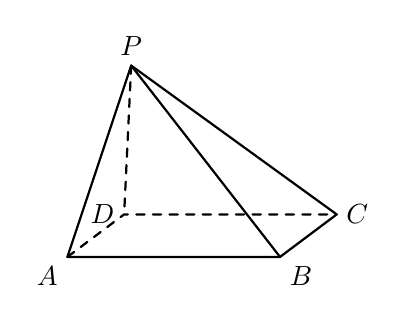
\begin{tikzpicture}[>=stealth,scale=0.9,line cap=round,line join=round]
  \coordinate (A) at (0,0);
  \coordinate (B) at (3,0);
  \coordinate (D) at (0.8,0.6);
  \coordinate (C) at (3.8,0.6);
  \coordinate (P) at (0.9,2.7);
  \draw[thick] (A)--(B)--(C)--(P)--cycle;
  \draw[thick] (P)--(B);
  \draw[thick,dashed] (A)--(D)--(C);
  \draw[thick,dashed] (P)--(D);
  \node[below left] at (A) {$A$};
  \node[below right] at (B) {$B$};
  \node[right] at (C) {$C$};
  \node[left] at (D) {$D$};
  \node[above] at (P) {$P$};
\end{tikzpicture}
\end{center}
\nopagebreak[4]
\Needspace{4\baselineskip}
\textbf{解析}

底面矩形面积为 $AB\cdot AD=3$。因 $AB\perp AD$ 且 $PA\perp AB$，所以 $AB$ 垂直平面 $PAD$。在 $\triangle PAD$ 中，$PA=4$、$\angle PAD=60^\circ$，点 $P$ 到底面的高为 $PA\sin60^\circ=2\sqrt3$。故 $V=\dfrac13\cdot3\cdot2\sqrt3=2\sqrt3$。

\Needspace{5\baselineskip}
在平面 $PAD$ 内从 $P$ 向 $AD$ 作垂线，垂足 $E$ 落在 $AD$ 的延长线上；$AE=PA\cos60^\circ=2>AD$，且 $PE=PA\sin60^\circ=2\sqrt3$。在底面内过 $E$ 作 $EF\parallel DC$，交 $BC$ 的延长线于 $F$，则 $EF=DC=AB=3$。由三垂线定理，$PF\perp BC$，因此 $\angle PFE$ 是二面角 $P-BC-D$ 的平面角。在直角三角形 $PEF$ 中，
\nopagebreak[4]
\[
\tan\angle PFE=\frac{PE}{EF}=\frac{2\sqrt3}{3},
\]
故二面角大小为 $\arctan\dfrac{2\sqrt3}{3}$。
\nopagebreak[4]
\begin{center}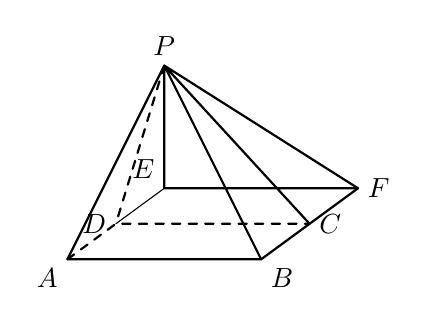
\begin{tikzpicture}[>=stealth,scale=0.82,line cap=round,line join=round]
  \coordinate (A) at (0,0);
  \coordinate (B) at (3,0);
  \coordinate (D) at (0.75,0.55);
  \coordinate (C) at (3.75,0.55);
  \coordinate (E) at (1.5,1.1);
  \coordinate (F) at (4.5,1.1);
  \coordinate (P) at (1.5,3.0);
  \draw[thick] (A)--(B)--(F);
  \draw[thick,dashed] (A)--(D)--(C);
  \draw[thick,dashed] (P)--(D);
  \draw[thick] (P)--(A) (P)--(B) (P)--(C) (P)--(E) (P)--(F) (E)--(F);
  \draw[thin] (D)--(E);
  \node[below left] at (A) {$A$};
  \node[below right] at (B) {$B$};
  \node[right] at (C) {$C$};
  \node[left] at (D) {$D$};
  \node[above left] at (E) {$E$};
  \node[right] at (F) {$F$};
  \node[above] at (P) {$P$};
\end{tikzpicture}
\end{center}
\nopagebreak[4]
\gkanswer{答案：$V=2\sqrt3$；二面角大小为 $\arctan\dfrac{2\sqrt3}{3}$。}

\end{answer}
\begin{answer}
\gksolhead{24}{答案见下}

\textbf{题目}：

（本题满分 18 分，共 2 个小题，第 1 小题满分 6 分，第 2 小题满分 12 分。）设椭圆的方程为 $\dfrac{x^2}{m^2}+\dfrac{y^2}{n^2}=1$（$m,n>0$），过原点且倾角为 $\theta$ 和 $\pi-\theta$（$0<\theta<\dfrac\pi2$）的两条直线分别交椭圆于 $A,C$ 和 $B,D$ 四点。（1）用 $\theta,m,n$ 表示四边形 $ABCD$ 的面积 $S$；（2）若 $m,n$ 为定值，当 $\theta$ 在 $(0,\dfrac\pi4]$ 上变化时，求 $S$ 的最大值 $u$。

\Needspace{4\baselineskip}
\textbf{解析}

\Needspace{5\baselineskip}
令 $t=\tan\theta$。直线 $y=tx$ 与椭圆的交点横坐标满足
\nopagebreak[4]
\[
\frac{x^2}{m^2}+\frac{t^2x^2}{n^2}=1,
\quad x^2=\frac{m^2n^2}{n^2+m^2t^2}.
\]
\Needspace{5\baselineskip}
对应纵坐标绝对值为 $t|x|$。四边形面积为
\nopagebreak[4]
\[
S=4|xy|=\frac{4m^2n^2t}{n^2+m^2t^2}
=\frac{4m^2n^2\tan\theta}{n^2+m^2\tan^2\theta}.
\]

对 $t\in(0,1]$，函数导数的符号由 $n^2-m^2t^2$ 决定。若 $n\le m$，最大值在 $t=n/m$（等号情形 $t=1$）处取得，$u=2mn$。若 $n>m$，函数在 $(0,1]$ 上递增，最大值在 $t=1$ 处取得，$u=4m^2n^2/(m^2+n^2)$。当 $m=n$ 两式一致，均为 $2m^2$；卷内分段写法遗漏了等号边界，答案在此补明。

\gkanswer{答案：（1）$S=\dfrac{4m^2n^2\tan\theta}{n^2+m^2\tan^2\theta}$；（2）$n<m$ 时 $u=2mn$，$m<n$ 时 $u=\dfrac{4m^2n^2}{m^2+n^2}$。题面还允许 $m=n$；此时两式均给 $u=2m^2$，分段边界在原答案中未列。}

\end{answer}
\begin{answer}
\gksolhead{25}{答案见下}

\textbf{题目}：

（本题满分 18 分，共 3 个小题，第 1 小题满分 4 分，第 2 小题满分 6 分，第 3 小题满分 8 分。）已知二次函数 $y=f(x)$ 在 $x=\dfrac{t+2}{2}$ 处取得最小值 $-\dfrac{t^2}{4}$（$t\ne0$），$f(1)=0$。（1）求 $y=f(x)$ 的表达式；（2）若任意实数 $x$ 都满足等式 $f(x)g(x)+mx+n=x^3$（$g(x)$ 为多项式），试用 $t$ 表示 $m$ 和 $n$；（3）设 $t=-3$，圆 $C_k$ 的方程为 $(x-mq^k)^2+(y-nq^k)^2=r_k^2$（$0<q<1,r_k>0$），圆 $C_k$ 与 $x$ 轴相切，圆 $C_k$ 与 $C_{k+1}$ 外切（$k=0,1,2,\ldots$），记 $S$ 为所有这些圆的面积之和，求 $q,S$ 的值。

\Needspace{4\baselineskip}
\textbf{解析}

\Needspace{5\baselineskip}
（1）设 $f(x)=a\left(x-\dfrac{t+2}{2}\right)^2-\dfrac{t^2}{4}$。代入 $f(1)=0$ 得 $a\,t^2/4-t^2/4=0$。因 $t\ne0$，所以 $a=1$，从而
\nopagebreak[4]
\[
f(x)=x^2-(t+2)x+t+1=(x-1)(x-t-1).
\]

\Needspace{5\baselineskip}
（2）在恒等式 $f(x)g(x)+mx+n=x^3$ 中分别代入 $x=1$ 与 $x=t+1$，得到
\nopagebreak[4]
\[
m+n=1,\qquad (t+1)m+n=(t+1)^3.
\]
因 $t\ne0$，解得 $m=t^2+3t+3$、$n=-t^2-3t-2$。

\Needspace{5\baselineskip}
（3）令 $t=-3$，则 $m=3,n=-2$，圆心为 $(3q^k,-2q^k)$。圆与 $x$ 轴相切且半径为正，故 $r_k=2q^k$。相邻圆心距为 $\sqrt{13}\,q^k(1-q)$。外切条件给出
\nopagebreak[4]
\[
2q^k+2q^{k+1}=\sqrt{13}\,q^k(1-q),
\quad q=\frac{\sqrt{13}-2}{\sqrt{13}+2}.
\]
\Needspace{5\baselineskip}
所有圆的面积和为
\nopagebreak[4]
\[
S=\sum_{k=0}^{\infty}\pi r_k^2
=4\pi\sum_{k=0}^{\infty}q^{2k}
=\frac{4\pi}{1-q^2}
=\pi\left(2+\frac{17\sqrt{13}}{26}\right).
\]

\gkanswer{答案：（1）$f(x)=x^2-(t+2)x+t+1$；（2）$m=t^2+3t+3$，$n=-t^2-3t-2$；（3）$q=\dfrac{\sqrt{13}-2}{\sqrt{13}+2}$，$S=\pi\left(2+\dfrac{17\sqrt{13}}{26}\right)$。}

\end{answer}